\documentclass{article}

\usepackage[utf8]{inputenc}
\usepackage{ctex}
\usepackage{assignpkg}
\usepackage{amsmath}
\usepackage{amssymb}

\usepackage{ifthen}
\usepackage{tikz}

\studentIds{202XX80XXXXXXXX}
\studentNames{XXX}

\assignmentNumber{}

\date{\today}
\usepackage{hyperref}
\begin{document}
\usetikzlibrary{calc}
\makecover%\chapter*{}

\section{简要介绍}
本文是阅读文献\href{https://ieeexplore.ieee.org/stamp/stamp.jsp?tp=&arnumber=1676518}{Decrypting a Class of Stream Ciphers Using Ciphertext Only}后的一些个人感受和总结。其中这篇文章主要针对的是基于线性移位寄存器和非线性函数的某类伪随机数发生器($pn$)的攻击。该攻击利用的是随机数发生器的输出、为其提供输入的某个线性移位寄存器($LFSR_i$)的输出、密文之间可能存在的相关性。
\section{攻击原理}
%\alpha=
\begin{figure}[htbp]
\centering
	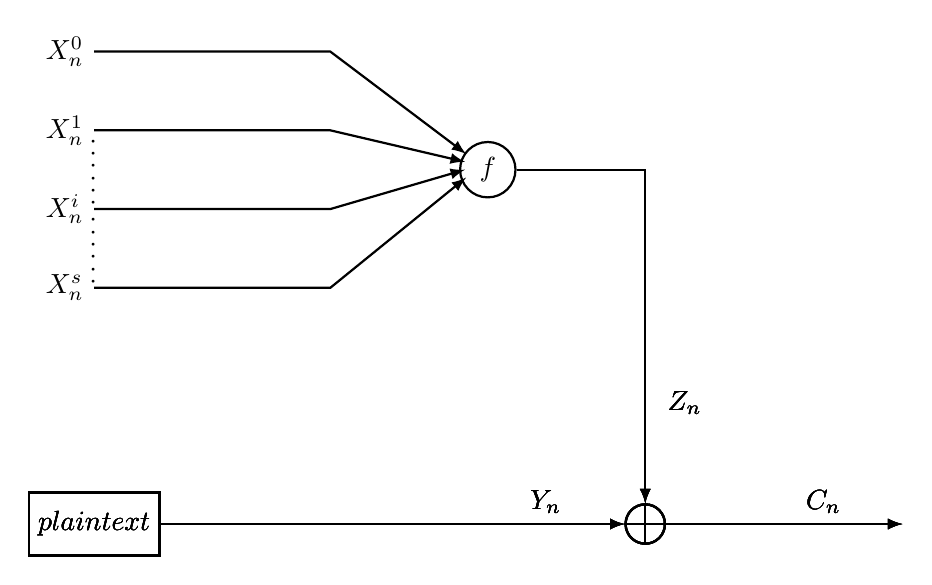
\begin{tikzpicture}[thick]
	\node (nlf) [circle, minimum size=0.5cm, draw=black] at (5,-1.5) {$f$};
	\foreach \i/\j in {0/0,1/1,2/i,3/s}{
		\draw[-latex] (0, -\i) node [left] {$X_n^\j$} -- (3, -\i) -- ( [xshift=(\i*\i*0.05-\i*0.15+0.6)*0.15 cm, yshift = (2-\i) * 0.1 cm]nlf.west);
		\ifthenelse{\i=1 \OR \i=2}{
			\node [rotate=90] at (0, -0.5 - \i) {$\cdots \cdots$};
		};
	\node (BMS) [rectangle, minimum width=1cm, minimum height=0.8cm,draw=black] at (0,-6) {$plaintext$};
	\node (XOR) [circle, minimum size=0.5cm,draw=black] at (7,-6){};
	\draw[-] (XOR.west)--(XOR.east);
	\draw[-] (XOR.north)--(XOR.south);
	\draw[-latex] (BMS.east) -- (XOR.west) node [left=1cm, above] {$Y_n$};
	\draw[-latex] (XOR.east) -- ([xshift=3cm]XOR.east) node [left=1cm, above] {$C_n$};
	\draw[-latex] (nlf.east) -- (7, -1.5) -- (XOR.north) node [right=0.5cm, above=1cm] {$Z_n$};
	};
	\end{tikzpicture}
	\caption{流密码系统的输入输出数据模型}
\end{figure}
上图是描述该流密码加密系统得到第$n$个密文比特$C_n$的数据模型。其中
\begin{itemize}
	\item 
	$C_n$:密文的第$n$比特
	\item 
	$Y_n$:明文的第$n$比特
	\item 
	$Z_n$:随机数生成器输出的第$n$比特,也就是密钥的第$n$比特。其中随机数生成器=$s$个线性移位寄存器+非线性函数$f$。
	\item 
	$X_n^i$:第$i$个线性移位寄存器$LFSR_i$输出的第$n$比特,
\end{itemize}
该系统利用随机数生成器($pn$)生成密钥流,并将明文与密钥流异或得到密文。
\subsection*{密钥比特的生成}
随机数发生器包含两个部分,第一部分是$s$个线性移位寄存器,它们每人贡献出$1$比特$X_n^i$作为第二部分非线性函数$f$的输入,所以非线性函数$f$的输入是$s$个比特,其输出是一个比特。这一比特$Z_n$作为密钥的第$n$位。
\subsection*{该密码系统被破解的判断条件}
该系统的密钥就是那个随机数发生器,因为非线性函数$f$是已知的,所以我们只需要破解和$s$个线性移位寄存器有关的部分就行了。而线性移位寄存器中最关键的就是它们的初始序列状态以及它们的反馈连接方式。
$LFSR_i$的初始序列状态和反馈连接方式,我们称之为部分密钥$LFSR_i$。所以我们需要做的就是确定部分密钥$LFSR_i$。

这里所说的反馈连接方式,指的可能是实际的线性反馈移位寄存器电路的连接方式,而某种连接方式是对应着某个本原多项式的。具体言之,一个$m$级线性反馈移位寄存器的反馈连接方式的个数等于$m$次本原多项式的个数。

\subsection*{攻击复杂度}

%其中,$LFSR_i$的级数(也可以说是其长度)为$r_i$,产生的序列的周期为$2^{r_i}-1$(每一个序列产生的都是$m$序列,也就是$LFSR$的特征多项式都是本原多项式),所以序列的初态$s_{i}$共有$2^{r_i}-1$种。
为了破解这个密码系统,我们不仅要知道每个线性移位寄存器的连接方式,还需要每个寄存器的初态。

首先分析单个线性移位寄存器有多少种可能的状态。
对于单独某个线性反馈移位寄存器$LFSR$,设其级数为$r$,其可能使用的本原多项式的个数为$R$个,那么这个线性移位寄存器$LFSR$有$R(2^r-1)$个可能的状态。
(因为它使用的是本原多项式,所以产生的序列是$m$序列,而每个本原多项式产生的$m$序列都有$2^{r}-1$种状态)


对于前述密码系统中的线性反馈移位寄存器$LFSR_i$,我们设其级数为$r_i$,其可能使用的本原多项式的个数为$R_i$个。

假如用穷举攻击破解该密码系统,我们需要同时破解这个$s$个线性移位寄存器,那么其复杂度(也就是密钥空间的复杂度)为:
\[K=\prod_{i=1}^{s}R_i(2^{r_i}-1)\]

假如我们可以通过某种方法将这$s$个线性移位寄存器分而治之,逐个击破(即首先确定$LFSR_i$的状态,再确定$LFSR_2$的状态,……)那么攻击的复杂度就变成了
\[\sum_{i=1}^{s}R_i(2^{r_i}-1)\]

$LFSR_i$可能存在的$R_i(2^{r_i}-1)$种状态中,有一种状态是密码系统中随机数发生器生成密钥时$LFSR_i$的状态,也就是对应于$LFSR_i$部分的正确密钥。假如我们能找到这个状态区别于其他剩余状态的特征,并能利用该特征将这个状态找出来,那就好办了。而这个特征就是相关性。
% 那么$LFSR_i$有多少种可能的状态呢?
% 首先由于其使用本原多项式,故其产生的序列是$m$序列,共有$2^{r_i}-1$种。而由于其可能使用不同的特征多项式

% 也就是说真实的部分密钥$LFSR_i$是$R_i(2^{r_i}-1)$个状态中的某一种,那我们只要找到这个真实密钥区别于其他不是真实密钥的某一个特征,并利用该特征将真实密钥找出来就行了。(下文将对该特征进行更加详细的描述。)

% 于是要破解该密码系统,则需要破解同时破解这个$s$个线性移位寄存器,那么穷举攻击的复杂度(也就是密钥空间的复杂度)为:
% \[K=\prod_{i=1}^{s}R_i(2^{r_i}-1)\]
% 但是通过相关攻击,可以将这个$s$个线性移位寄存器分而治之,逐个击破,也就是说逐个地破解部分密钥$LFSR_i$,所以该攻击的复杂度变成了破解每个部分密钥$LFSR_i$的复杂度的加和:
\subsection*{相关性}
首先思考一个问题,就是非线性函数$f$的第$i$个输入$X_n^i$和$f$的输出$Z_n$存在相关性吗?它们可能是彼此独立的、毫无关联的吗?不难想象,它们之间存在某种联系,存在相关性。

那么同样的,密文比特$C_n$和密钥比特$Z_n$存在相关性吗?略加思考,我们也会觉得他们存在相关。

那么,即然$X_n^i$和$Z_n$相关,$C_n$和$Z_n$相关,那么我们也可以认为$X_n^i$和$C_n$相关。

经过一系列的推导,在原论文中最终得到的表明$X_n^i$和$C_n$存在的联系是
$P(C_n \oplus X_n^i = 0) = 1 - p_0 - q_i + 2p_0q_i$。其中
\begin{itemize}
	\item 
	$p_0$:明文比特为0的概率,即$p_0=P(Y_n=0)$;该概率依赖于明文,认为是可计算出来的常数;
	\item
	$q_i$:非线性函数的输出$Z_n$与其第$i$个输入相等的概率,即$q_i=P(Z_n=X_n^i)$,该概率依赖非线性函数,可以认为是一个常数;
\end{itemize}

设$A,B$分别表示某一比特,$A\oplus B=0$在密码学中还是相当常见的,根据本人的理解,$A\oplus B=0$等价的意思是$A=B$,也就是说比特A和比特B相等。那么反之,$A \oplus B = 1$的意思就是$A\neq B$。

文中引入的判断$X_n^i$与$C_n$相关性的量是$\alpha_0=\sum_{n=1}^{N}(1-2(C_n \oplus X_n^i))$。怎么理解这个量呢?我们可以看到:
\begin{itemize}
	\item 
	$C_n \oplus X_n^i = 0$:即$C_n$与$X_n^i$相等,$\alpha_0$将增加一;
	\item
	$C_n \oplus X_n^i = 1$:即$C_n$与$X_n^i$不等,$\alpha_0$将减少一;
\end{itemize}

也就是说,$\alpha_0$的值就是$N$对比特(第$n$对为$C_n$和$X_n^i$,注意这里下标$n$才是$N$的迭代变量,$X$的上标$i$的含义是表明我们在研究第$i$个线性移位寄存器与$C_n$的关系)中,$C_n$和$X_n^i$相等的次数减去$C_n$和$X_n^i$不等的次数。

可想而知,我们在研究第$i$个线性移位寄存器时,我们随意选择一个初态和一个本原多项式,如果它恰好是产生正确密钥的那个初态和那个本原多项式,那么$\alpha_0$的值就相对来说比较大。如果它不是正确密钥,那么$\alpha_0$相对来说比较小。

那么我们就选择能产生最大的那个$\alpha_0$的初态和本原多项式来作为正确密钥吗?这样肯定是不行的,毕竟正确密钥下的$\alpha_0$更大,只是一个高概率事件,概率高不代表它就一定会发生。
\subsection*{阈值$T$的引入}
那么我们可以怎么做呢?
我们设置一个阈值$T$,
\begin{itemize}
\item
如果$\alpha_0>T$,则我们把$\alpha_0$对应的那个初态和连接方式设置成正确密钥的候选密钥。也就是说,我们认为这个密钥可能是正确的密钥。这种情况下,我们接受了原文的假设$H_1$,即$\alpha_0$是$X_n^i$和$C_n$的相关函数。
\item
如果$\alpha_0 \leq T$,则我们就认为$\alpha_0$对应的那个初态和连接方式不是正确的。也就说我们排除了这个密钥是正确密钥的可能性。这种情况下,我们接受了原文的假设$H_0$,即$\alpha_0$不是$X_n^i$和$C_n$的相关函数。

\end{itemize}
%将$\alpha_0$值大小超过某一阈值$T$的部分密钥$LFSR_i$(下文简称密钥)作为正确密钥的候选密钥,

对于候选密钥,我们还需要进行额外的测试来判断它是不是正确密钥(比如更换别的密文,看它是不是以很高的概率比我们所选的阈值$T$大)。

%最糟糕的情况下,就是正确密钥恰好是你要尝试的部分密钥$LFSR_i$中的最后一个,那么你就要进行大约$R_i(2^{r_i})$次尝试。

引入这个阈值$T$之后,会不会出现什么问题呢?

比如说我在一次测试中,刚好正确密钥产生的$\alpha_0$小于我设置的阈值$T$,那我就与正确的密钥失之交臂了。我希望这件事情$(\alpha_0 < T | H_1)$不会发生。也就是说,我希望这件事情发生的概率很低。所以我想知道$P_m=P(\alpha_0<T | H_1)$的概率有多大。

同时我们还希望,错误的密钥产生的$\alpha_0$满足$\alpha_0>T$这件事$(\alpha_0>T | H_0)$发生的概率也不要太大。最好是一次也不发生在我测试的过程中一次也不发生。如果这个概率很大的话,我就有很多候选密钥,我就要做很多额外的测试。
所以我还想知道$P_f=P(\alpha_0>T | H_0)$有多大。
% \begin{itemize}
% \item
% 我刚好把正确密钥给排除了
% \item
% 我把一个错误的密钥设置成了
% \end{itemize}

为了求出上述两件事情的概率,我们要知道正确密钥下$\alpha_0$的分布和错误密钥下$\alpha_0$的分布,根据中心极限定理,原文推导出
\begin{itemize}
	\item 
	正确密钥下的$\alpha_0$的分布:数学期望为$N(2p_e-1)$,方差为$4N(1-p_e)p_e$的正态分布。
	\item 
	错误密钥下的$\alpha_0$的分布:数学期望为$0$,方差为$N$的正态分布。对应于原文中添加的那个$X_n^0$
\end{itemize}

根据原文的推导,我们知道
\begin{equation}
\left\{
\begin{aligned}
&P_m=Q(|\gamma_0|)\\
&P_f=Q(|\sqrt{N}(2p_e-1)-2\gamma_0\sqrt{p_e(1-p_e)}|)
\end{aligned}
\right.
\end{equation}


\subsection*{$T$和$N$的选取}

%因为我希望错误的密钥产生的$\alpha_0$满足$\alpha_0>T$这件事发生的概率很低,低到我$R_i(2^{r_i})$次测试过程中这件事都不会发生一次,也就是说$P_f \leq \frac{1}{R_i(2^{r_i})}$。

那么$T$和$N$怎么选取呢?这里$N$指我们需要比较多少比特的密文$C_n$和$X_n^i$。这里就涉及到我一个知识的盲区了,原文在选取$T$和选取$N$的时候,他说道,``For a chosen value $P_m$'',其中$P_m$是正确密钥下比较$C_n$和$X_n^i$得出的$\alpha_0$小于阈值$T$的概率。个人感觉$P_m$大小不能控制,所以无法被选取,所以也不太理解。

后来我仔细一想,认为是这么个意思:他在进行对密钥破解前,首先明确自己这次破解过程中希望$P_m$大概是多大,然后在设置了这个$P_m$值的大小的前提下来依次设置另外两个参数——需要比较的比特位数$N$和阈值$T$。

而在设置$N$值的大小时,他希望在错误密钥下比较$C_n$和$X_n^i$得出的$\alpha_0$值大于$T$的概率很低,低到在所有$R_i2^{r_i}$次尝试中只发生一次。即$P_f = \frac{1}{R_i2^{r_i}}$。

于是通过确定$P_f$的值该取多大,就可以确定$N$的值该取多大。

确定$N$之后,那么根据原文的公式
\[P_m= Q[|\frac{N(2p_e-1)-T}{2\sqrt{N}\sqrt{p_e(1-p_e)}}|]\]
阈值$T$也就被唯一的确定了。

也就是说,我们在明确了自己希望的$P_m$和$P_f$的取值之后($P_m$是一开始就选好的一个攻击参数,$P_f$的大小被限定为$\frac{1}{R_i2^{r_i}}$),我们可以唯一确定$N$和$T$的大小。
\section{攻击结果}
在攻击结果中,原文给出了两张图,Fig. 8是为了检验$Z_n$(注意,这里是随机数生成器$Z_n$,而不是密文$C_n$)和$X_n^i$存在相关关系。检验也是通过比较$Z_n$和$X_n^i$而得到一个和之前一样的$\alpha_0$值(这个值应该也就是原文中的CCF, cross-correaltion function,$\alpha_0$的分布应该是数学期望为$N(2q_i-1)$,方差为$4Nq_i(1-q_i)$),观察并得到事件$\alpha_0>T$的概率分布图,图中的横纵坐标貌似都进行了归一化。可以看出该图像形似与用1减去正态分布的分布函数$F(x)$的函数图像$y=1-F(x)$。这里大多是猜测,可能对图像的理解不够准确。

Fig. 7给的是在攻击中,正确密钥下计算出来的$\alpha_0$绝对值超过错误密钥值得到的$\alpha_0$值的最大值的两倍。说明$\alpha_0$值确实是可以区分正确密钥和错误密钥的特征,攻击效果不错。

\end{document}
